\begin{surferPage}[Quintic (15 Cusps)]{Quintic s 15 vrhova}
	Ploha stupnja $5$ (quintic) ima $15$ singulariteta tipa $A_2$ (zovemo ih vrhovi). 
	Ova ploha, kao i niz povezanih ploha, su objavljene u \v clanku iz 2005.\ godine, a 
	autor je Oliver Labs.
	Pet vrhova se vidno razlikuju od preostalih deset.
	Zaista, ovih pet vrhova su $A_2^{++}$ singulariteti, a ostalih deset su $A_2^{+-}$ 
	singulariteti (pogledajte galeriju o jednostavnim singularitetima za vi\v se informacija):
	
	 \vspace*{-0.3em}
    \begin{center}
      \begin{tabular}{c@{\qquad}c}
        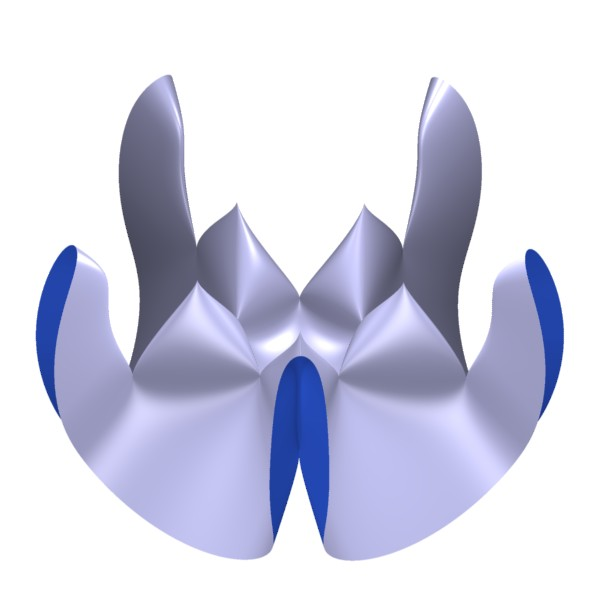
\includegraphics[height=1.2cm]{./../../common/images/dessins_quint_15a2}
        &
        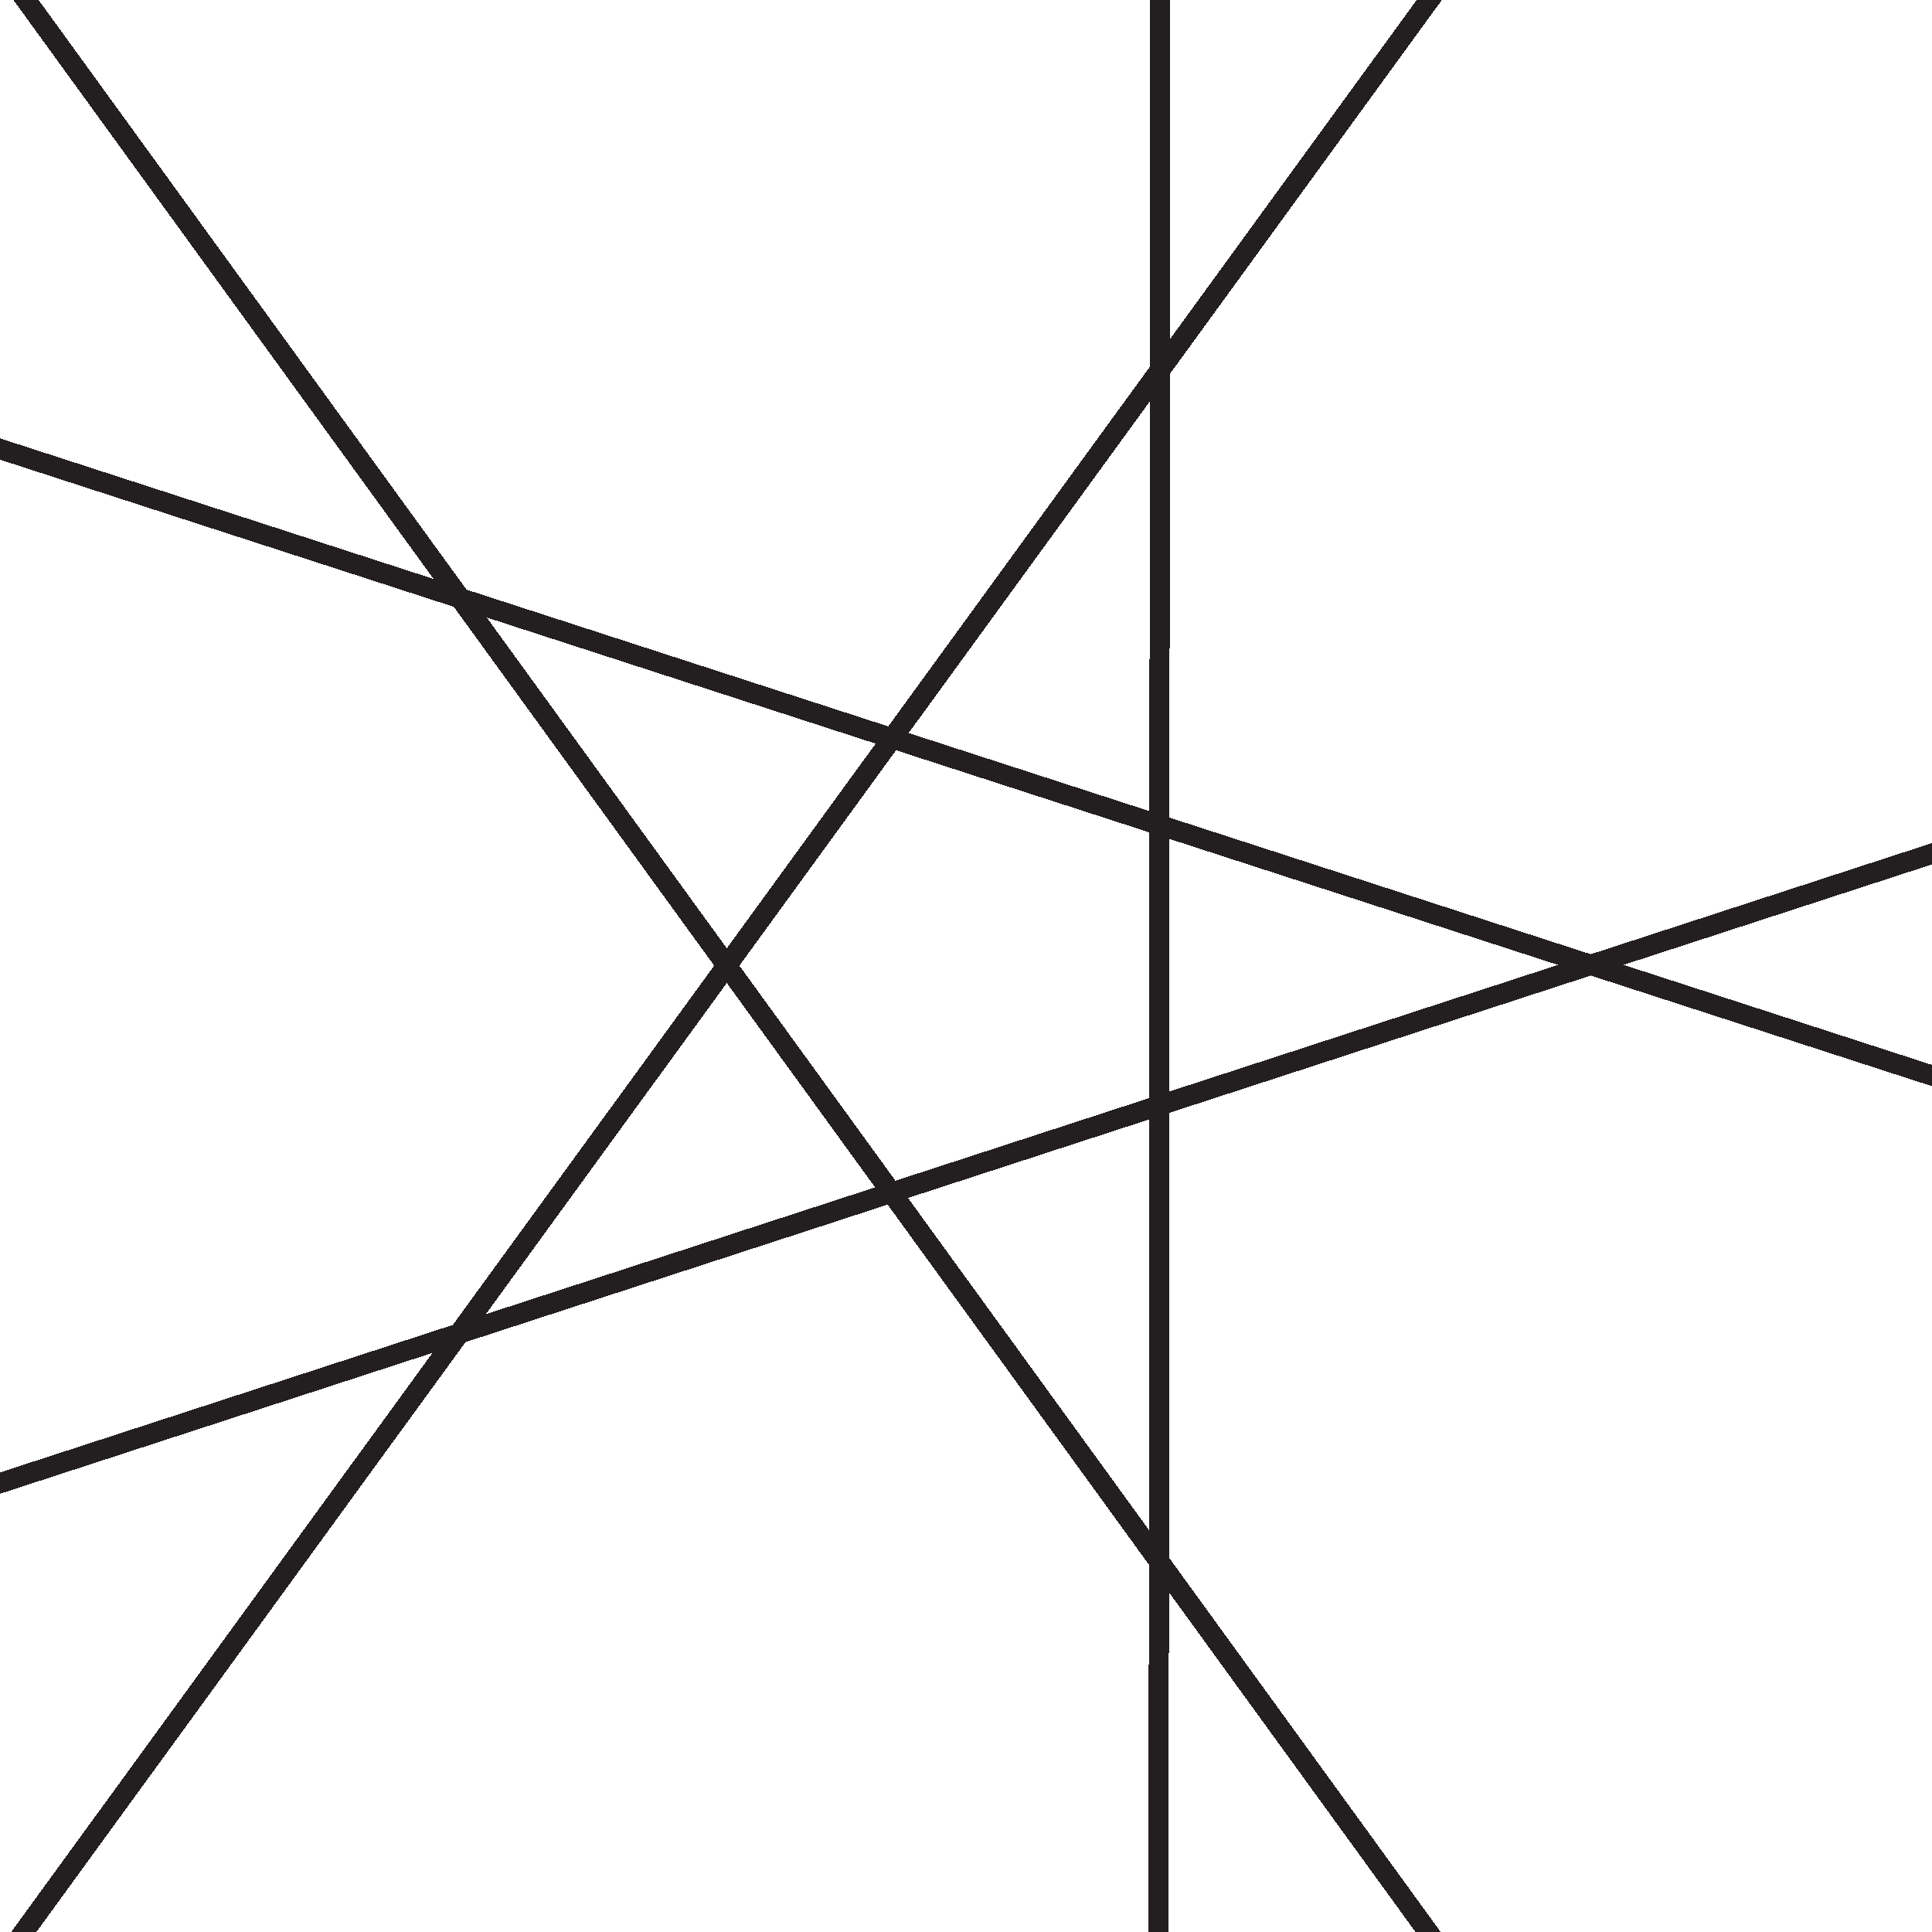
\includegraphics[height=1.2cm]{./../../common/images/rp5.pdf}
      \end{tabular}
    \end{center}
    \vspace*{-0.3em}    
		
		Ova ploha ima jednad\v zbu oblika
		$S_5(x,y) + t(z)=0,$ 
		gdje je $S_5(x,y)$ pravilni peterokut (desna slika), a $t(z)$ je 
		varijanta \v Cebi\v sevljevih polinoma koje smo ve\' c spomenuli nekoliko puta.
		
		 Jo\v s jedan quintic s $15$ vrhova (lijevo) je konstruirao Wolf Barth. Taj 
		quintic je, kao \v sto mo\v zemo vidjeti iz slike u sredini, povezan s 
		plohom Clebsch Cubic (desno):
		
		\vspace*{-0.3em}
    \begin{center}
      \begin{tabular}{c@{\quad}c@{\quad}c}
        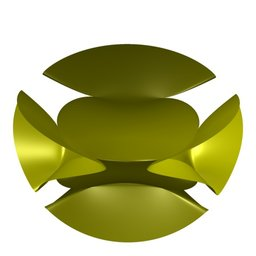
\includegraphics[height=1.2cm]{./../../common/images/barthquintic_green}
        &
        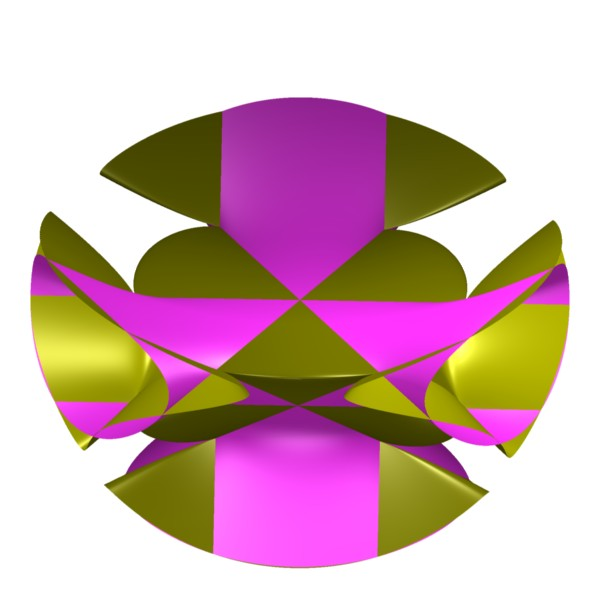
\includegraphics[height=1.2cm]{./../../common/images/barthquintic_clebschcubic}
        &
        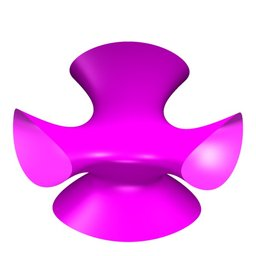
\includegraphics[height=1.2cm]{./../../common/images/clebschcubic_pink}
      \end{tabular}
    \end{center}
    \vspace*{-0.3em}
\end{surferPage}
